\documentclass[a4paper]{article}
\usepackage[utf8]{inputenc}
\usepackage[T1]{fontenc}
\usepackage{textcomp}
\usepackage{amsmath, amssymb, amsthm}
\usepackage{geometry}
\usepackage{tikz-cd}
\usepackage{mdframed}
\usepackage{microtype}
\usepackage{hyperref}
\usepackage{cleveref}

\usepackage[backend = biber, style = alphabetic]{biblatex}
\addbibresource{../references.bib}

% figure support
\usepackage{import}
\usepackage{xifthen}
\usepackage[textsize=tiny,colorinlistoftodos,obeyDraft]{todonotes}
\newcommand{\question}[1]{\todo[color=green!40]{#1}}
\usepackage{pdfpages}
\usepackage{transparent}
\newcommand{\incfig}[1]{%
	\def\svgwidth{\columnwidth}
	\import{./figures/}{#1.pdf_tex}
}

\pdfsuppresswarningpagegroup=1


\newcommand{\N}{\mathbb{N}}
\newcommand{\Z}{\mathbb{Z}}
\newcommand{\Q}{\mathbb{Q}}
\newcommand{\C}{\mathbb{C}}
\newcommand{\R}{\mathbb{R}}
\newcommand{\F}{\mathbb{F}}
\newcommand{\pro}{\mathbb{P}}
\newcommand{\aff}{\mathbb{A}}
\newcommand{\ltr}{\par \noindent \framebox[1\width]{ $\implies$ } \hspace{.2cm}}
\newcommand{\rtl}{\par \noindent \framebox[1\width]{ $\impliedby$ } \hspace{.2cm} }

\DeclareMathOperator{\coker}{coker}
\DeclareMathOperator{\id}{Id}
\DeclareMathOperator{\im}{Im}
\DeclareMathOperator{\spec}{Spec}
\DeclareMathOperator{\maxspec}{MaxSpec}
\DeclareMathOperator{\spf}{Spf}
\DeclareMathOperator{\proj}{Proj}
\DeclareMathOperator{\red}{red}
\DeclareMathOperator{\trop}{trop}
\DeclareMathOperator{\trdeg}{TrDeg}
\DeclareMathOperator{\divisor}{Div}
\DeclareMathOperator{\cov}{Cov}

\newcommand{\into}{\hookrightarrow}
\newcommand{\onto}{\twoheadrightarrow}
\newcommand{\divides}{\mid}
\newcommand{\notdivides}{\nmid}
\newcommand{\Gan}{\ensuremath{\mathbb{G} _m ^{\mathrm{an}}}}
\newcommand{\an}{{}^{\text{an}}}
\newcommand{\cox}{\widehat{\otimes}}

\newcommand{\st}{%
  \nonscript\;
  \ifnum\currentgrouptype=16
    \,\middle|\,
  \else
    \,|\,
  \fi
  \nonscript\;}

\theoremstyle{definition}
\newtheorem{definition}{Definition}[subsection]
\newtheorem{remark}[definition]{Remark}
\newtheorem{theorem}[definition]{Theorem}
\newtheorem{example}[definition]{Example}
\newtheorem{lemma}[definition]{Lemma}
\newtheorem{claim}[definition]{Claim}
\newtheorem{proposition}[definition]{Proposition}
\newtheorem{exercise}[definition]{Exercise}
\newtheorem{corollary}[definition]{Corollary}


\author{Micha\"el Maex}


\title{Mid year report: Berkovich Geometry}

\begin{document}

\maketitle

\tableofcontents

\pagebreak

\section{Introduction} \label{sec:introduction}

A powerful tool to study complex varieties is the analytification functor, which turns a variety over $\C$ into a complex manifold, that then can be studied using analytic method. 
Other rings that are well suited for analysis are the $p$-adic fields $\Q_p$ or more generally non-archimedean fields. 
So the question arises whether a similar analytification functor can be constructed for  varieties over non-archimedean fields. 

Tate constructed the theory of rigid spaces as suitible analytic spaces. But they're various topological problems that makes them less than ideal. For example they are totally disconnected. To solve these problems Tate restricted the set of open and covers on these spaces. 

Berkovich proposed another approach by adding many more points to the rigid space to resolve various problem. 
The resulting topological spacse are very well behaved. For connected schemes they are path connected, compact. Even more, the analitification of a curve has the structure of a profinite real graph. 

For the thesis the main interest is not to do analysis on Berkovich spaces of varities, but rather to study the relation between the berkovich space of a curve and its semi-stable models as outlined in \cite{bakerStructureNonarchimedeanAnalytic2013}

This text is a based on various roughly analogous introductionary text on Berkovich geometry \cite{bakerarizona,temkinIntroductionBerkovichAnalytic2010,nicaiseNONARCHIMEDEANGEOMETRY,boschLecturesFormalRigid2014}. 

\section{Basic valuation theory} \label{sec:basic_valuation_theory}

Let $R$ be any ring. On rings like $\Z$ and $\Q$ and $\C$ the absolute value function gives away of measuring how low \emph{large} each element is. 
These types of functions are called (semi)norms, absolute values or valuations. 
\begin{definition}
	Let $R$ be a ring. A \emph{absolute value on $R$} is a function $|\cdot |: R \to \R^{+}$ satisfying for all $a, b \in R$
	\begin{enumerate}
		\item $|a| = 0 \iff a = 0$ 
		\item $|a \cdot b| = |a| \cdot |b|$ 
		\item $|a + b| \le |a| + |b|$
	\end{enumerate}
\end{definition}
Note that $R$ is not the zero ring, then $|1| = 1$ because $|1|^2 = |1| $ and $|1|\ne 0 $. 
\begin{example}
	The usual definition of absolute value on $\Z, \Q, \R$ is an absolute value. 
\end{example}
\begin{example}
	On any ring we can define the trivial absolute value as \[
	 |a| = \begin{cases}
		 1 & a \ne 0 \\
		 0 & a = 0
	 \end{cases}
	.\] 
\end{example}
\begin{example}
	A weirder absolute value on $\Z$ is the \emph{$p$-adic absolute value}, where $p$ is a prime. 
	Its defined as $|a|_p = p^{-n}$ where $n$ is the largest integers such that $p^{n} \divides a$, if $a \ne 0$ and $|0|_p = 0$. 


	This $p$-adic absolute value can be extended to an absolute value on $\Q$ by defining $|a / b|_p = \frac{|a|_p}{|b|_p}$. Let $\frac{a}{b}$ be any fraction. 
	I like to think about this in the following way. 
	Factor out the largest powers of $p$ out of $a$ and $b$ and write $a = p^{n} a', b = p^{m} b'$. Then $\frac{a}{ b} = p^{n - m} \frac{a'}{ b'}$ and $|a / b|_p = p^{m - n}$. 
	So the $p$-adic absolute values only cares about what powers of $p$ occur and doesn't care about numbers coprime to $p $.
\end{example}
As we will see in \cref{sec:berkovich_spectrum_of_Z}, we have esssentially listed all absolute values on $\Z$ and $\Q$ as examples above.  

Absolute values are a special case of (semi)norms
\begin{definition}
	Let $R$ be any ring. A \emph{seminorm on $R$} is a function $|\cdot |: R \to \R^{+}$ satisfying for all $a, b \in R$ 
	\begin{enumerate}
		\item $|0| = 0, |1| = 1$ 
		\item $|a \cdot b| \le |a | \cdot |b|$  (submultiplicativity)
		\item $|a + b| \le |a + b|$ (triangle inequality)
	\end{enumerate}
	A seminorm is called \emph{multiplicative} if it also satisfies a stronger version of 2. 
	\begin{enumerate}
		\item [4.]  $|a \cdot  b| = |a | \cdot |b|$
	\end{enumerate}
	A seminorm that is only satisfies $2$ is sometimes called a \emph{submultiplicative seminorm} if we need to stress that the norm is not required to be multiplicative. 
\end{definition}

\begin{definition}
	The \emph{kernel} of a seminorm $|\cdot |: R \to \R^{+}$ is defined as \[
		\ker(|\cdot |) = \{a \in \R \st |a| = 0\} 
	.\] 
\end{definition}
\begin{remark}\label{rem:ker_norm_ideal}
	Let $ |\cdot |$ be a norm on $R$. Then $\ker |\cdot |$ is an prime ideal of $R$. If $|\cdot |$ is multiplicative then $\ker |\cdot |$ is even a prime ideal!
\end{remark}
\begin{proof}
	Let $a, b \in \ker |\cdot |, c \in R$. Then $0 \le |a + b| \le |a|+|b| = 0$. So  $a + b \in \ker |\cdot |$. 
	Also $0 \le |c \cdot a| \le |c|\cdot |a| = 0$. So $c \cdot a \in \ker |\cdot |$. 
	This shows that $\ker |\cdot  |$ is an ideal. 
	
	Suppose that $|\cdot |$ is multiplicative. 
	Let $a, b\in R $ such that $a\cdot b \in \ker |\cdot |$ then  $|a|\cdot |b| = |a\cdot b| = 0$. 
	Hence either $|a| = 0$ or  $|b|=0$. 
	So either  $a \in \ker |\cdot |$ or $b \in \ker |\cdot |$. 
\end{proof}

In some sense seminorms are analogous to ideals and and multiplicative seminorsm are analogous to prime ideals. This is will be the basis of Berkovich spectra of Rings.
Like the ordinary $\spec$ functor we can define the space of all multiplicative norms on a ring. 
But hold your horses trying to define a suitable zarisky topology on this space. 
That won't work. 
In fact we will need two different topologies on this space for the theory to work. 
Don't worry, this is a feature, not a bug. 
One topology will have all the nice properties you can think of: Haussdorf, compact, path-connected, locally contractible, \ldots while the other one is great for sheaf theory. 


\begin{definition}
	Let $R$ be a ring and $|\cdot |$ are seminorm. 
	Then $|\cdot |$ is called a \emph{norm} if $\ker |\cdot | = 0$, i.e.\ $|a| = 0 \iff a = 0$. 
\end{definition}

So an absolute value is a multiplicative norm. 

\begin{lemma}
	Any seminorm $|\cdot |$ on a field $F$ is a norm, i.e.\ has trivial kernel. 
\end{lemma}
\begin{proof}
	We have that $|1| = 1$. So $1 \not\in \ker |\cdot |$ and thus $\ker |\cdot |$ is an ideal of $F$ different from $F$. 
	As $F$ is a field this means that $\ker |\cdot | = (0)$. So $|\cdot |$ is norm. 
\end{proof}

\begin{definition}
	A (semi)norm $\|\cdot \|$ on $R$ is called \emph{non-archimedean} if it satisies the following stronger version of the triangle inequality, \[
	\forall a, b \in \R: \|a + b\| \le \max \{\|a\|, \|b\|\} 
	.\] 

	Confusingly a \emph{Archimedean (semi)norm} is a norm that is not non-archimedean.
\end{definition}

\begin{exercise}[\cite{nicaiseNONARCHIMEDEANGEOMETRY}]
	Let $k$ be a field.
	Show that a absolute value  $|\cdot |$ on $k$ is non-Archemedean if and only if the image of $\Z$ in $k$ is bounded. 
\end{exercise}
\begin{proof}
	Suppose $|\cdot |$ is non-archimedean. Then for any positive integers $n$ we have \[
	|n| = \left|\sum_{i = 1}^{n} 1 \right| \le \max \{1, 1, \ldots, 1\}  = 1
	.\] 
	And for negative integers we have $|n| = |-n| \le 1$. So $\|\cdot \|$ is bounded on the image of $\Z$ by $1$. 


	Suppose that $|\cdot |$ is bounded on the image of $\Z$ by $c$. 
	Let $x, y \in k$. Then \[
		|(x + y)^{n}| = \left| \sum_{i = 0}^{n} \binom{i}{n} x ^{i} y ^{n-i}\right| \le n\cdot c \max(x, y)^{n}
	.\] 
	So \[
		|x + y| \le \sqrt[n]{c\cdot n}  \max(x, y)
	.\] 
	Taking $n \to \infty$ yields the non-archimedean triangle inequality. 
\end{proof}

\begin{corollary}
	Let $A \subset  B$ an inclusion of rings  equipped with multiplicative such that the norm on $B$ extends the norm on $A$. 
	Then $A$ is non-archimedean if and only if $B$ is non-archimedean. 
\end{corollary}

\begin{remark}
	Suppose $R$ is non-archimedean and we have $a, b \in R$ such that $|a| \ne |b|$ then the triangle inequality is an equality \[
	|a + b| = \max \{|a|, |b|\} 
	.\] 
	So in some sense equality is the generic case. 
\end{remark}
It may sound like a really strong property to have, and that not many norms will be non-archimedean. 
But as you will see in this thesis, most norms that pop up are non-archimedean. 
In fact the only complete valued fields with archimedean norms are $\R$ and $\C$ \todo{find reference}.



\begin{definition}
	equivalent norm\todo{define this}
	{\color{red} This is a problem because equivalent norms and equivalent valuations are different as far as I understand}
\end{definition}

Note that the definition a non-archimedean norm only depends on the multiplicative structure on $\R^{+}$ and no longer depends on the additive structure. 
Sometimes it is more natural define norms in terms the isomorphic group $\R, +$. 
These are typically called valuationas. 


\begin{definition}
	Let $R$ be a ring. A valution on $R$ is a function $v:R \to \R \cup \{\infty\} $ such that 	
	\begin{itemize}
		\item $v(0) = \infty$, $v(1) = 0$. 
		\item $v(a\cdot b) = v(a) + v(b)$
		\item $v(a + b) \le \min\{v(a), v(b)\}$
	\end{itemize}
\end{definition}

\begin{remark}
	Note that there is essentially no difference between a non-archimedean absolute value and a valuation because one can take for absolute value $|\cdot |$ defines a valution $x \mapsto -\log |x|$ and a valution $v$ defines a non-archimedean absolute value $x\mapsto e^{- v(x)}$. 
\end{remark}



\subsection{Non-Archimedean rings and fields} \label{sec:non-archimedean_rings_and_fields}


\begin{theorem}\label{thm:norm_finite_field_ext}
	If $L$ is a finite field extension of a complete non-archimedean field $K$, then there is a unique extension of the norm of $K$ to $L$ and this extension is also non-archimedean.
\end{theorem}
\begin{proof}
	This a very technical result and for the proof we refer to \cite[][appendix A]{boschLecturesFormalRigid2014}. 
\end{proof}

\begin{corollary}
	If $K$ is a complete non-archimedean field then the norm of  $K$ extends uniquely to its algebraic closure $\overline{K}$.
\end{corollary}
\begin{proof}
	Recall that \[
	\overline{K} = \varprojlim_{L \supset K} L
	.\] 
	where $L$ ranges over all algebraic extensions of $K$. 
	As all these algebraic extensions have unique norms extending  the norm on $K$ and for $L_1 \supset L_2 \supset K$ the norm on  $L_1$ must restrict to norm on $L_2$ by uniqueness, it is clear that the norm functions $L \to \R^{+}$ glue to a map $\|\cdot \|: \overline{K} \to \R^{+}$. 

	It is easy to verify that this is a norm on $\overline{K}$ extending the norm on $K$. 
\end{proof}

\begin{theorem}
	[Krasner's Lemma]
	Let $K$ be a non-archimedean algebraically closed field. 
	Then its completion, $\widehat K$ is algebraically closed as well. 
\end{theorem}
\begin{proof}
	This follows from the continuity of roots. See \cite[][lem A.6]{boschLecturesFormalRigid2014} for a detailed argument. 
\end{proof}

This show that we can cannonically turn any non-archimedean field $K$ into an algebraically closed field by considering $\widehat{\overline{K}}$, which is first taking the algebraic closure of $K$ and then completing it. 

\begin{definition}
	For a prime $p$ we define the \emph{p-adic complex numbers} as \[
	\C_p = \widehat{\overline{\Q_p}}
	.\] 
\end{definition}

This is useful because Berkovich geometry works best when the base field is algebraically closed and complete. 

\begin{definition}
	Let $R$ be a non-archimedean ring. Then we write 
	\begin{align*}
		R^{0} &= \{a \in k \st |k| \le 1\}  \\
		R^{00} &=  \{a \in k \st |k| < 1\}  \\
		\tilde R &= R^{0} / R^{00}
	.\end{align*}
\end{definition}
If $k$ is a field then $k^{0}$ is a valuation ring and $ k^{00}$ is its maximal ideal. 

We will useally write $K$ for a non-arcimedean field, $R = K^{0}$ for its valuation ring, $k = \tilde K$ for its residue field. 

\begin{definition}
	Let $K$ be a non-archimedean ring. 
	The \emph{value group of $K$} is \[
	|K| = \{|a| \st \} 
	.\] 
\end{definition}


\subsection{Ultrametric spaces} \label{sec:ultrametric_spaces}

\begin{definition}
	A \emph{ultrametric space} is a topological spaces $(X, d)$ where the metric satisfies the non-archimedean triangle inequality. 
	\[
		d(x, y) \le \max \{d(x, z) ,d(z, y)\}, \quad \forall x, y ,z \in X
	.\] 
\end{definition}
\begin{exercise}
	If $d(x,z) \ne d(z,y)$ the inequality is an equality. 
\end{exercise}
\begin{proof}
	Suppose without loss of generality that $d(x, z) \ge d(z,y)$, so $d(x, y) \le \max \{d(x, z), d(z,y)\} = d(x, z) $. 
	Then $d(x, z) \le \max \{d(x, y), d(y,z)\}$. So $d(x, z) \le d(x, y) \le d(x, z)$. So we find equality.
\end{proof}
\begin{corollary}
	Any point of a ball (open or closed) is a center for that ball. 
\end{corollary}
\begin{corollary}
	If two balls have non-empty intersection that one must be included in the other. 
\end{corollary}
\begin{corollary}
	The topology of $X$ is totally disconneced. 
\end{corollary}

Non-archimedean fields are ultrametric spaces with the metric $d(x, y) = |x - y|$. 



\section{Berkovich Spaces of rings} \label{sec:berkovich_spaces}


I will introduce a preliminary definition of the Berkovich spectrum of a ring, which for now will just be a topolgoical space. 
It will serve build intuition for Berkovich spaces by exploring the Berkovich spectrum of two rings $\Z$ and $K[T]$ where $K$ is a complete algebraically closed field. 

\begin{definition}
	Let $A$ be a ring. Then we define \[
		\mathcal{M} (A) = \{x: A \to \R^{+} \st \text{multiplicative seminorm on } A\} 
	.\] 
	This comes equipped with the coarsest topology such that for every $a \in A$ the map $\mathcal{M} (A) \to [0, \infty) : \|\cdot \|_x \mapsto \|f\|_x $ is continuous. 

	We will almost always deal with a relative case where $A$ is a $k$-algebra over some real valued field $K$. In this case adjust the definition \[
		\mathcal{M} (A) = \{x : A \to \R^{ + }  \mid \text{multiplicative seminorm on }A \text{ extending the norm on } K\} 
	.\] 
	Again $\mathcal{M} (A)$ comes with the coarsest topology making all maps $\mathcal{M} (A) \to [0, \infty): x \mapsto \|a\|_x, \forall a \in A$ continuous. 
\end{definition}
We think of $\mathcal{M} (A)$ as a geometric space and thus its elements are points, usually denoted by a letter, like $x$. 
For an element $f \in A$ we write $|f|_x$ or $x(f)$ for  $f$ evaluated in the norm $x$. 

\begin{remark}
	$\mathcal{M}$ is not only a map, but it is also a contravariant functor. 
	Let $A, B$ be two rings and $f: A \to B$ a morphism. 
	Then a seminorm $x \in \mathcal{M} (B)$ turns into a seminorm on $\mathcal{M} (A)$ by defining $\mathcal{M} (f)(x): A \to \R^{ +}: a \mapsto |f(a)|_x$.


This is analogous to the $\spec$ functor and there even is a natural transformation $\mathcal{M} \implies \spec$ defined by $\mathcal{M} (A) \to \spec A: |\cdot |_x \mapsto \ker x$. This is well defined by \cref{rem:ker_norm_ideal}. 
\end{remark}

There also is a generalisation of the residue field at a prime ideal. 

\begin{definition}\label{def:completed_residue_field}
	Let $A$ be a ring (possibly over $K$) and $x \in \mathcal{M} (A)$ a point in its Berkovich spectrum. 
	Then the \emph{completed residue field at $x$} is defined as \[
		\mathcal{H} (x) = (A / \ker x, |\cdot |_x)^{\wedge}
	.\] 
	This is the completion of $A / \ker x$ with respect to the norm induced by $x$. 
	It comes with a induced morphism $\chi_x: A \to \mathcal{H} (x)$.
	\question{its not really necessary to take the kernel here right? Completing will already do that because they will be equivalent cauchysequences?}
\end{definition}

Like $\spec$, the points in $\mathcal{M} $ can be described as \emph{characters}, i.e.  maps $\chi: A \to L$ (over $K$) where $L$ is a complete valued field subject to the condition that $\chi_1: A \to L_1, \chi_2: A \to L_2$ are equivalent if there exists another map to a complete valued field $\chi: A \to L$  and maps $L \to L_1, L \to L_2$ extending the norm on $L$ such that the diagram 
\[
\begin{tikzcd}
	& A \ar{dl}[']{\chi_1} \ar{dr}{\chi_2} \dar{\chi} \\
	L_1 & L \lar \rar & L_2
\end{tikzcd}
\] 
commutes. 
For any point $x$ the map $\chi_x: A \to \mathcal{H} (x)$ gives a minimal representative for the character corresponding to the point $x$. 


\begin{remark}
	Later we will consider other topologies on $X\an$, which will be necessary to turn $X\an $ into a ringed space. 
	There topologies will not be topologies like we know it. They will be Grothendieck topologies, where which unlike ordinary topologies restrict the notion of a cover. 
\end{remark}

\begin{proposition}\label{prop:spec_ring_haussdorf}
	Let $R$ be a ring then $\mathcal{M} (R)$ is Haussdorf. 
\end{proposition}
\begin{proof}
	Let $x, y \in \mathcal{M} (R)$ be two different points. 
	Then there is some $f \in R$ such that $f(x) \ne f(y)$. 
	So there are opens $U_x, U_y \subset  [0, \infty)$ that separate $f(x), f(y)$.
	Recall that $\phi: \mathcal{M} (A) \to [0, \infty): x \mapsto f(x)$ is continuous by definition of the topology on $\mathcal{M} (A)$. 
	So $\phi^{-1}(U_x)$ and $\phi^{-1}(U_y)$ are opens in $\mathcal{M} (R)$ separating $x,y$. 
\end{proof}


\subsection{The Berkovich spectrum of $\Z$} \label{sec:the_berkovich_spectrum_of_z}
Classyfing all norms on $\Z$ was already done by Ostrowski.
\begin{theorem}[Ostrowski]\label{thm:ostrowksi}
	Any multiplicative norm $|\cdot |'$ on $\Z$ is either
	\begin{itemize}
		\item \emph{the trivial norm} \[
				|\cdot |_0: n \mapsto \begin{cases}
					1 & n \ne 0 \\
					0 & n = 0
				\end{cases}
			\]
		\item an \emph{archimedean norm} \[
				|\cdot |_{\infty, \epsilon}: n \mapsto |n|^{\epsilon},
			\]
			for $0 <  \epsilon \le 1$
		\item a \emph{$p$-adic norm} \[
				|\cdot |_{p, \epsilon}: t \mapsto \epsilon ^{- v_p(t)},
			\]
			for $p$ a prime numbers and $0 < \epsilon < \infty$. 
		\item a $p$-adic trivial seminorm 
			\[
			|\cdot |_{p, \infty}: n \mapsto \begin{cases}
				1 & p \nmid n \\
				0 & p \mid n
			\end{cases}
			,\] 
			for $p$ prime. 
	\end{itemize}
\end{theorem}
So for every $p \in \{\text{primes}\} \cup \{\infty\} $ we find a continuous family of norms \[
	\epsilon \mapsto|\cdot |_{p, \epsilon}
\] 
for $\epsilon \in [0, 1]$ if $p = \infty$ and else $\epsilon \in [0, \infty]$. 
When $\epsilon = 0$ these all give the trivial norm. 
So these rays glue together at at point and the Berkovich space $\mathcal{M} (\Z)$ looks like \cref{fig:berkovich-space-of-z}.
We have to be careful with the topology here. 
While each of branches is homemorphic to a closed interval, they are not glued together along an open. 
So the topology is not uniquely determined by the topology of each branch separately.
In fact, any open containing the point $|\cdot |_0$ has to contain all but finitely many of the branches. 

\begin{figure}[h]
    \centering
    \incfig{berkovich-space-of-z}
    \caption{berkovich space of $\Z$}
    \label{fig:berkovich-space-of-z}
\end{figure}


It is a good exercise to verify that 
\begin{itemize}
	\item  $\mathcal{H}(|\cdot |_0) = \Q$ 
	\item $\mathcal{H} (|\cdot |_{\infty, \epsilon}) = \R$ for $\epsilon \in (0, 1]$
	\item $\mathcal{H} (|\cdot |_{p, \epsilon}) = \Q_p$ for $\epsilon \in (0, \infty)$
	\item $\mathcal{H} (|\cdot |_{p, \infty}) = \F_p$ 
\end{itemize}
While it may seem like the completed residue field of different norms can be the same, it is actually not as they will be equipped with different norms.  


\subsection{Berkovich specturm of $\aff^{1}_K$} \label{sec:berkovich_specturm_of_affine_line}


For the rest of this document we will let $K$ be a fixed complete algebraically closed non-archimedean field with non-trivial absolute value. We write 
\begin{align*}
	R &:= K^{o} = \{a \in K \st |a| \le 1\} \\
	\mathfrak{m}  &:= K^{oo} =  \{a \in K \st |a| < 1\}  \text{ the unique maximal ideal of } R\\
	k &:= \widetilde K = R / \mathfrak{m} \text{ the residue field of } R
.\end{align*}
Note that $k$ is automatically algebraically closed as well. 

\medskip

We will describe the Berkovich space of the polynomials in one variable  $\mathcal{M} (K[T])$ where $K$ like usual is an algebraically closed, complete field which is not trivially-valued. 
We will call this $\aff_K^{1}\an$, the analityfication of the affine line. 

One way to find norms on $K[T]$ would taking a point $a \in K$ and define $|f|_a = |f(a)|_K$ where $|\cdot |_K$ is the norm on $K$. 
So there is a natural embedding $K \into \mathcal{M}(K[T])$ and we often implicitly identify these points.  

Another way to define a norm is by choosing a closed disk $B(a, r) = \{x \in K \st |x - a| \le r\} $ with center $a$, and radius $r$ and define \[
	|f|_{B(a, r)} = \sup_{x \in B(a, r)} |f(x)|
.\] 
\begin{claim}
	The norm $|f|_{B(a, r)}$ as defined above is a well defined multiplicative seminorm extending the norm on $K$. 
	If $r \in |K|$ then the sumpremum is a maximum and the maximum is obtained for some point on the boundary of $B(a, r)$.
\end{claim}
\begin{proof}
	Let $f = \sum_{i = 0}^{n} a_i T^{i}$. 
	Then for $x \in B(a, r)$ we have $|x| \le |a| + r$. 
	So  $|f(x)| \le  \sum_{i = 0}^{n} |a_i| |x|^{i} \le \sum_{i = 0}^{n}|a_i| (|a| + r)^{i} $. 
	This last bound is indenpent of $x$. Hence the supremem exists. 

	Non-archimedean triangle inequality and extending the norm on $K$ is easily checked. 
	The multiplicativity is a little bit more suttle. 

	Without loss of generality we may translate the disk such that $a = 0$. 
	Lets assume for now that $r \in |K|$.
	Then we may also rescale such that $r = 1$. 

	Clearly the seminorm is multiplicative for elements in  $K$, i.e.\ for every $\lambda \in K, f \in K[t]: |\lambda \cdot f|_{B(a, r)} = |\lambda|\cdot |f|_{B(a, r)}$.  Let $f, g \in K[T]$, which we may rescale by an element of $K$, such that the largest coefficient of $f, g$ has norm $1$. In particular this means that $|f|_{B(0,1)}, |g|_{B(0,1)} \le 1$. 
	Then $f, g \in R[T]$ and their  reductions modulo  $\pi$ $\overline{f}, \overline{g} \in k[T]$ are nonzero.
	So $\overline{f}, \overline{g}$ have only a finite number of roots. In particular these is some $\overline{a} \in k$, represented by $a \in R$ such that $\overline{f}(\overline{a}) \ne 0, \overline{f}(\overline{a})\ne 0$. 
	Hence $f(a), g(a) \in R = B(0, 1)$ an $|f(a)| = |g(a)| = 1$. 
	So the supremem is obtained in $a$ for both polynomials and the norm is multiplicative as the supremem for $f\cdot g$ will also be obtained in $a$. 
\end{proof}

\begin{remark}\label{rem:norm_disk}
	From the proof above it follows that if $f = \sum_{i = 0}^{n} b_i (T-a)^{i}$ is the taylor expansion of $f$ around $a$ then for any $r$
	\[
		|f|_{B(a, r)} = \max_{i}\{  |b_i|r^{i}\}
	.\] 
\end{remark}
\question{Heeft dit een rigoreuser bewijs nodig?}


So the space of closed discs in $K$, which includes points (discs of radius zero), embeds as well in $\mathcal{M} (K[T])$. 
As we will see in a second these will make up almost all of the points on $\mathcal{M} (K[T])$. 
Ingoring these missed points, this means that $\mathcal{M}(K[T])$ is connected. 
Indeed, let $a \in K$ be any point. Then we can define a line \begin{equation}\label{eq:line_in_A_1}
	\ell_a: [0, \infty) \to  \aff_K^{1, \text{an}}: r\mapsto B(a, r)
\end{equation}
Because in an ultrametric space any point in a ball is a centre of ball, we see that for any two points $a, b$ the lines $\ell_a, \ell_b$ consinde for any $r \ge |a - b|$. 
So $\aff_K^{1,\text{an}}$ is not only connected, it is path connected!

We have been missing a few points on $\aff_K^{1, \text{an}}$. 
The Berkovich classification theorem gives all points. 
\begin{theorem}
	[Berkovich Classification theorem, \cite{bakerarizona}] 
	Any point $x \in \aff_K^{1,\text{an}}$ is given by decreasing sequences of closed disks $B_n = B(a_n, r_n)$ in $K$ by the formula \begin{equation}\label{eq:norm_disk_polynomial}
	|f|_x = \lim_{n \to \infty} |f|_{B_n}
	.\end{equation}
	Morover, two such sequences $B_n, B'_n$ define the same norm if and only if:
	 \begin{itemize}
		\item Both sequences have the same non-emtpy intersection, i.e.\ $\bigcap_{n = 1}^{\infty} B_n = \bigcap_{n = 1}^{\infty} B_n' \ne \emptyset$. 
			In this case the intersection $B = \bigcap_{n \in N} B_n$ is a closed disk (possibly a point) and $x = |\cdot |_B$. 
		\item Both sequences have empty intersection, i.e.\ $\bigcap_{n = 1}^{\infty} B_n = \bigcap_{n = 1}^{\infty} B_n' = \emptyset$  and for every $n$ there are $m, m'> n$ such that $B_n \supset  B'_{m'}$  and $B'_n \supset B_m $.
	\end{itemize}
	This means that we can classify the points in $\aff ^{1,\text{an}}_K$ into four types depending on $B = \bigcap_{n \in \N} B_n$. 
	\begin{description}
		\item[Type I:] $B = \{a\} $ a point and the $|f|_x = |f(a)|$. 
		\item[Type II:] $B = B(a, r)$ with $r \in |K^* |$ and $|f|_x = |f|_{B(a, r)}$
		\item[Type III:] $B = B (a, r)$ with $r \not\in |K^*|$ and $|f|_x = |f|_{B(a, r)}$
		\item[Type IV:] $B = \emptyset$
	\end{description}
\end{theorem}
As you can see our previous discussion has excluded type four points. We will see an example of such point in \cref{ex:type4point}. 

\begin{proof}
	I will only show the proof that every norm is given by such a sequence as the proofs of all other statements are technical and give little insight. 

	Let $x \in \aff_K^{1, \text{an}}$ be a multiplicative seminorm on $K[T]$. 
	As  $K$ is algebraically closed every polynomial factors into linear factors $(T-a)$. 
	Hence $x$ is uniquely detemrined by its value $|T-a|_x$ for each $a \in K$. 
	We will write $\rho_a = |T-a|_x$.
	Let  $a, b \in K$ such that $\rho_a \le \rho_b$. 
	Then  \begin{equation}\label{eq:proof_berk_class_1}
		|a - b|_x = |(T-b) - (T - a)|_x \le \max \{\rho_a, \rho_b\} = \rho_b 
	.\end{equation} 
	Hence $a \in B_{b, \rho_b}$ and thus  $B(a, \rho_a) \subseteq B(b, \rho_b)$. 

	Define $\rho := \inf_{a \in K} \rho_a$ and let $a_1, a_2, \ldots$ be a sequence such that $(\rho_{a_i})_{i \in \N}  $ is a non-increasing sequence converging to $\rho$. 
	By the previous remark this leads gives a decreasing sequence of disks \[
		B(a_1, \rho_{a_1}) \supset B(a_2, \rho_{a_2}) \supset B(a_3, \rho_{a_3}) \supset\ldots
	.\] 
	Now we will check that $|\cdot |_x = \lim_{n \to \infty} |\cdot |_{B(a_i, \rho_i)}$ by verifying that both norms agree on $T- b$ for every $b \in K$. 
	 There are two cases. Either $|T - b|_x = \rho_b = \rho$ or $\rho_b \ge \rho_{a_i}$ for some $i$. 

	 If $ \rho_b = \rho$ then by \eqref{eq:proof_berk_class_1} we find $|b - a_i|_x \le \rho_n$ for all $i$.
	 So \[
		 |T - b|_{B(a_i, \rho_i)} = |(T - a_i) - (b_i - a_i)|_{B(a_i, \rho_i)} = \max(\rho_n, |b - a_i|) = \rho_n
	 .\]
	 So $\lim_{i \to \infty} |T- b|_{B(a_i, \rho_i)} = \rho = |T - b|$. 

	 If $\rho_b > \rho$ then for $n \gg 0$ we have $\rho_b > \rho_a$ and thus $|b - a|_x \le \rho_b$, thus \[
		 |T - b|_{B(a_i, \rho_i)} = |(T - a_i) - (b -a_i)|_{B(a_i, \rho_i)} = \max (\rho_n, |b - a_i|) = |b - a_i| = |T - b|_x
	 .\]   
	 Taking the limit yields $\lim_{i \to \infty} |T- b| _{B(a_i, \rho_{i})} = |T - b|_x$.
\end{proof}

Using the Berkovich classification theorem, the properties about ultrametric spaces from \cref{sec:ultrametric_spaces} and a little imagination you can see that the $\mathcal{M} (K[T])$ looks something like \cref{fig:affine_line}. 
Points of type I-IV are highlighted in green. Note that the closed points of the curve $\spec K[T]$ are contained in  $\aff_K^{1,\text{an}}$ as exactly the type I points. 

\begin{figure}[h]
	\centering
	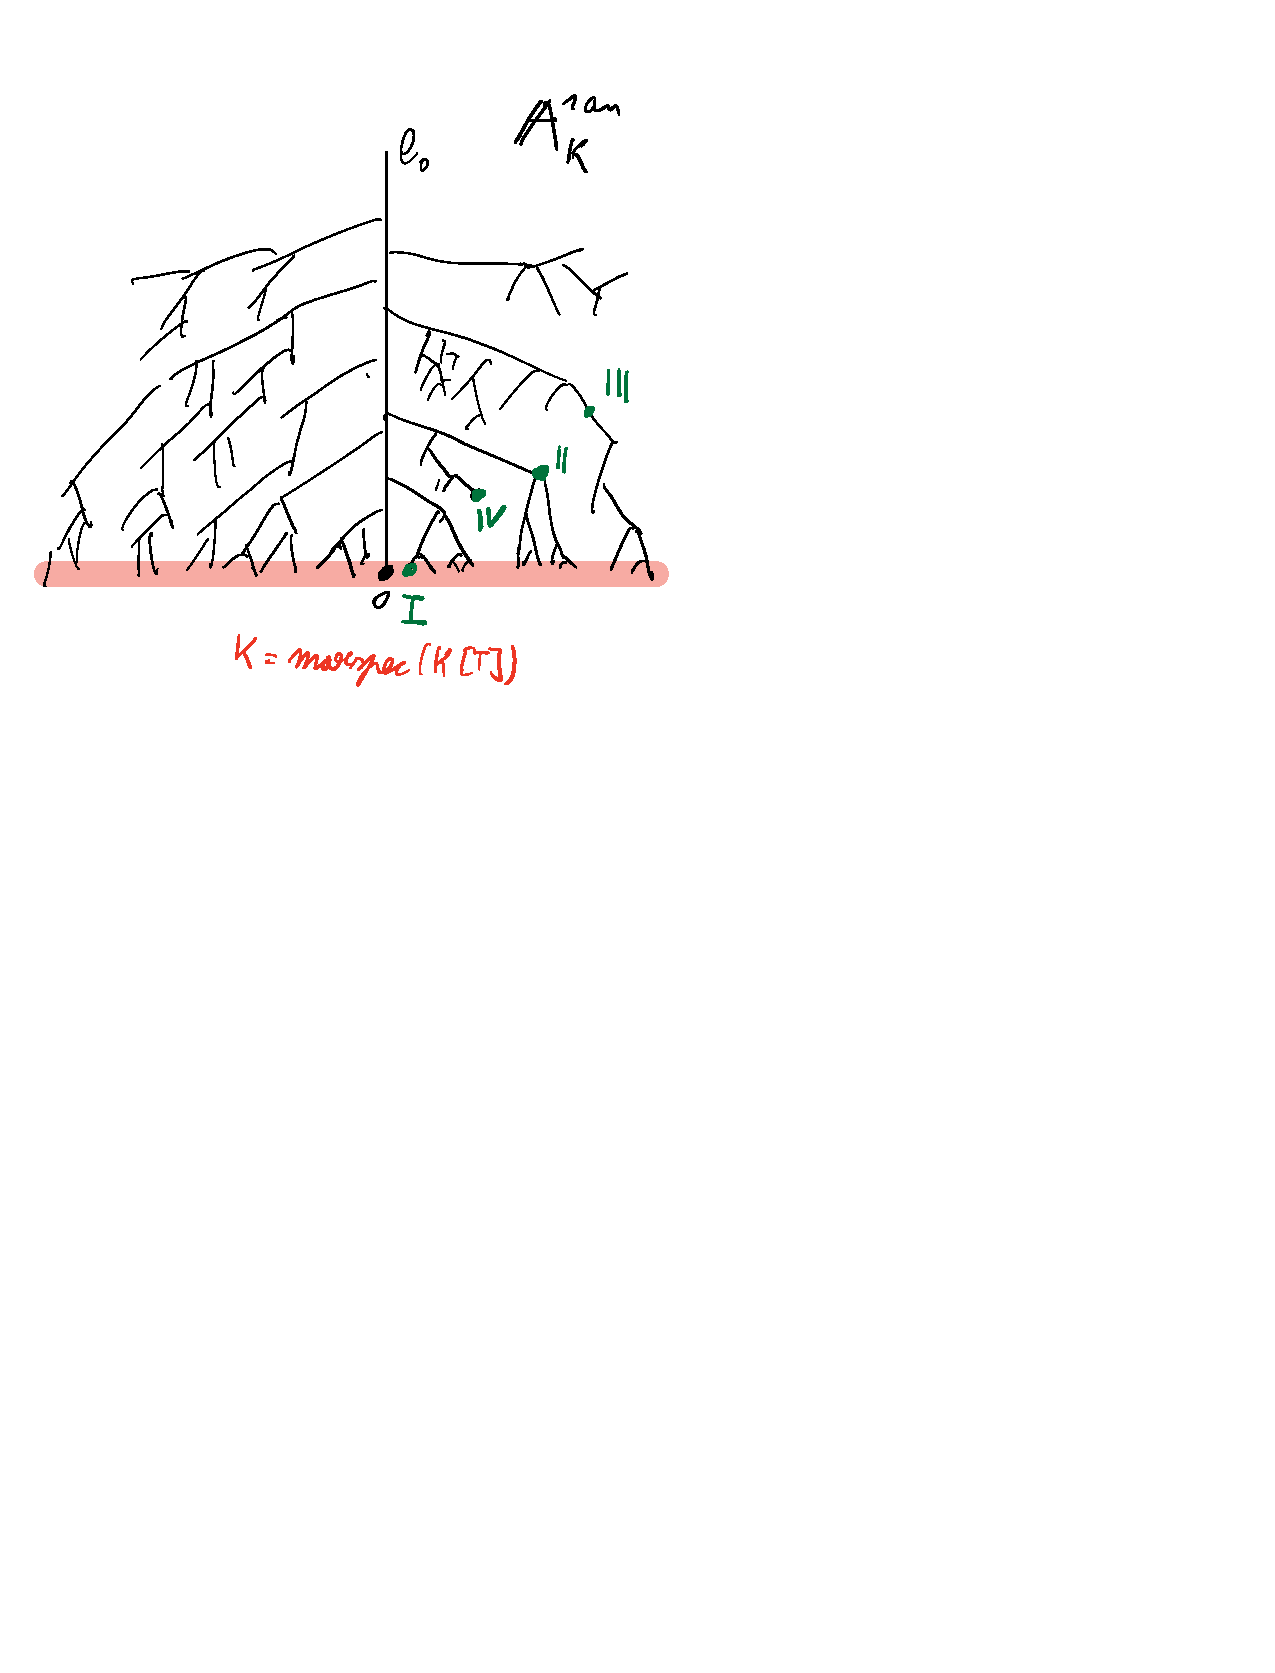
\includegraphics[width=0.5\textwidth]{figures/affine_line}
	\caption{The Berkovich affine line $\aff_K^{1, \text{an}} = \mathcal{M} (K[T])$, with the line $\ell_0$ from \cref{eq:line_in_A_1}}
	\label{fig:affine_line}
\end{figure}

There are other ways of recognizing type I, II, III and IV points, which will generalize better, when we look at Berkovich spectra of other curves. One is topological and the other one is purely algebraic. 

\begin{proposition}
	Let $x \in \aff_K^{1,\text{an}}$. 
	Let $C = \pi_0(\aff_K^{1, \an}\setminus \{ x\} )$ be the set of connected components the punctured affine line. 
	\begin{itemize}
		\item If $x$ is of type I  or IV then $C$ has only one element.
		\item If $x$ is of type II then there a natural morphism $C \simeq k \cup \{\infty\} $. Recall that $k = \tilde K = K^{o} / K^{oo} $. 
			So $x$ is an branch point where infinitely many branches connect. 
		\item If $x = |\cdot |_{B(a, r)}$ is of type III then $|C| = 0$. The two components are all disks containing $B(a, r)$ and all disks contained in $B(a, b)$. 
	\end{itemize}
\end{proposition}\question{Heeft het zin om hier een bewijs van te geven?}
\question{Zou het zinvoller zijn om tangents te definieeren als equivalentie klassen van paden vertrekkend uit een punt?}
The algebraic way to classify the points of $\aff_K^{1,\text{an}}$ is by using Abhyankar's inequality. 
\begin{definition}
	Let $K \subset L$ be a non-archimedean field extension. 
	Then we define \[
		E_{\frac{L}{ K}} = \dim \frac{|L^{\times }|}{|K^{\times }|} \otimes_\Z \Q, \qquad F_{L / K} = \trdeg(\tilde L / \tilde K)
	.\] 
\end{definition}

\begin{theorem}[Abhyankar inequality]
	Let $K \subset H \subset L$ be non-archimeadean rings extending each others norm. Assume that $L$ is algebraic over $\hat{H}$ and that $H$ is of trancendence degree $n$ over $K$. Then \[
	E_{L / K} + F_{L / K}  \le n
	.\] 
\end{theorem}

If $x \in \aff_K^{1, \text{an}}$ is a norm (not a seminorm) then its residue field $\mathcal{H} (x)$ is a completion on $K(T)$ with respect to the norm induced by $x$. As $K(T)$ is of trancendence degree 1 Abhyankar's inequality states that \[
	E_{\mathcal{H} (x) / K} + F_{\mathcal{H} (x) / K} \le 1
.\] 
This also allows us to classify points, because either both $E_{\mathcal{H} (x) / K}, F_{\mathcal{H} (x) / K}$ are zero, or exactly one is $1$. 
\begin{proposition}[2.3.3.3 in \cite{temkinIntroductionBerkovichAnalytic2010}]
	Let $x \in \aff_K^{1, \text{an}}$, then 
	\begin{itemize}
		\item $x$ is of type I if $\mathcal{H} (x) = K$
		\item $x$ is of type II if $F_{\mathcal{H} (x) / K} = 1$ and $E_{\mathcal{H} (x) / K} = 0$. 
		\item $x$ is of type III if $F_{\mathcal{H} (x) / K} = 0$ and $E_{\mathcal{H} (x) / K} = 1$.
		\item $x$ is of type IV if $\mathcal{H} (x) \subsetneq K$ and  $F_{\mathcal{H} (x) / K} = E_{\mathcal{H} (x) / K} = 0$.
	\end{itemize}
\end{proposition}

Type IV points are not rare. It might be counter intuitive that in a complete ring there exists a decreasing sequence of closed disks that has empty intersection. 
But in practice almost all fields have type  IV points. 
The trick is that the radii of these disks do not converge to $0$. 
\begin{example}[type IV point]\label{ex:type4point}
	Let $K = \C_p$ for some prime $p$. 
	Define 
	\begin{align*}
		a_n &= \sum_{i = 1}^{n} p^{-\frac{1}{n}}\\
		r_n &= p^{\frac{1}{n + 1}} \\
		B_n &= B(a_n, r_n) 
.\end{align*}
Then $|a_n - a_{n + 1}| = r_n$ and $r_{n + 1} \le r_n$ so the $B_{n + 1} \subset B_n$ and the sequence $(B_n)_n$ is decreasing. 
Now we have to show that the intersection $B = \bigcap_{i = 1} ^{\infty} B_n$ is non-empty. 

Let $x \in \C_p$. Then $x = \sum_{i = 0}^{m} b_i$ where $m$ is either finite or $m$ is infinite $b_i$ is a decreasing sequence such that $|b_i| \to 0$. Suppose that  $x \in B$, then $x \in B_n$ for every $n$, and thus we see that  $b_i = p^{\frac{-1}{i}}$ for any $i = 1, \ldots, n$.  
This is true for any $n $, so in particular we find that $b_i = p^{-\frac{1}{i}}$ for any $i$ .
But this contradicts that $b_i$ is unbounded. 
\todo{Make this more rigorous}
\end{example}



\section{$K$-analytic spaces} \label{sec:K_analytic_spaces}


In this section we'll describe the category of $K$-analytic spaces, which is where the Berkovich spaces of schemes will live. 
The main building blocks of these spaces are affinoid algebras which are a type of complete $K$-algebras. 
These will also be  crucial for defining the structure sheaf on Berkovich spaces. 

\subsection{Banach Algebras} \label{sec:banach_algebras}
\begin{definition}
	A $K$-Banach space is a $K$-vector space equipped with a norm that is complete with respect to that norm. 
\end{definition}

\begin{definition}
	Let $A, B$ be $K$-Banach spaces. 
	A $K$-vector space morphism $\phi: A \to B$ is \emph{bounded} if there is some $C\in \R$ such that $\|\phi(a)\|\le C \|a\| $. 
\end{definition}

\begin{lemma}
	A morphism $A \to B$ is bounded if and only if it is continuous. 
\end{lemma}

\begin{definition}
	A Banach $K$-algebra, $A$, is a commutative, associative, unital $K$-algebra with a submultiplicative norm that is a $K$-Banach space.
\end{definition}
\begin{definition}
	Let $A$ be a $K$-algebra. 
	Two norms $\|\cdot \|_1, \|\cdot \|_2$on $A$ are called equivalent if and only if they induce the same topology. 

	This means that there are non-zero constants $C, C'$ such that for every $ a\in A$ we have $C\|a\|_1 \le \|a\|_2 \le C'\|a\|_1$. 
\end{definition}

\begin{definition}
	Let $A$ be an $K$-Banach algebra and $I$ be a closed ideal in $A$. 
	Then we define the \emph{residue norm} on $A / I$ as 
	\begin{align*}
		\|\cdot \|_\text{res} : A / I &\longrightarrow \R \\
		a + I &\longmapsto \inf_{x \in a + I} \|x\|
	.\end{align*}
\end{definition}

To describe the category of $K$-Banach algebras we still need morphisms.
\begin{definition}
	Let $A, B$ be $K$-Banach algebras. 
	A $K$-algebra morphism $\phi: A \to B$ is \emph{admissible} if $\phi$ if the induced map $A / \ker \phi \to \im \phi$ is a homeomorphism, where $A / \ker \phi$ is equipped with the residue norm and $\im \phi$ with subspace norm of $B$. 
\end{definition}
\question{is admissible equivalent met bounded/continuous?}

\begin{remark}\label{rem:uniqueness_norm_banach_algebra}
	Note that the identity  $\id: (A, \|\cdot \|_1) \to (A, \|\cdot \|_2)$ between two Banach $K$-algebras is a isomorphism in the category of $K$-Banach spaces if and only if the norms $\|\cdot \|_1, \|\cdot \|_2$ are equivalent. 
	So the norm is not intrinsic to an equivalence class of objects in the category of Banach  $K$-algebras, but it is well defined up to equivalence. 
\end{remark}

There is also a good way to equip the tensor product of Banach $K$-algebras with a submultiplicative norm, turning is again into a Banach $K$-algebra.
\begin{definition}
	Let $A, B, C$ be Banach $K$-algebras with morphisms  $C\to A, C \to B$. Then the \emph{completed tensor product}, written $A \widehat \otimes_C B$, is the completion of the ordinary tensor product $A \otimes_C B$ with norm defined by \[
		\|x\| = \inf \left\{\max_{i = 1}^{n} |a_i||b_i|  \st n \in \N, a_i \in A, b_i \in B, x = \sum_{i = 1}^{n} a_i \otimes_C b_i\right\} 
	\] 
	for any $x \in A \otimes_C B$. 
\end{definition}
\question{Is dit tensor product altijd goed gedefinieerd? Of hebben we extra voorwaarden nodig op $A, B, C$?}

\begin{proposition}\label{prop:universal_prop_complete_tensor}
	The completed tensor product is the pushout of the diagram $A \leftarrow C \to B$ in the category of  $K$-Banach algebras. I.e.\ it satisfies the universal property that for any  $D$ and morphism $A \to D$,  $B \to D$ making the square with $C$ commute there exists a unique map $A \widehat\otimes_C B \to D$ making the diagram commute\[
	\begin{tikzcd}
		C \rar \dar & A \dar \ar[bend left]{rdd} \\
		B \rar \ar[bend right]{drr} &  A \widehat{\otimes}_C B \ar[dashed]{dr}{\exists !} \\
		 & & D
	\end{tikzcd}
	.\] 
\end{proposition}
\begin{proof}
	See \cite[][section 2.1.7]{siegfriedboschNonArchimedeanAnalysisSystematic1984}. 
\end{proof}

\subsection{Berkovich spectra of Banach algebras} \label{sec:berkovich_spectra_of_banach_algebras}


To an affinoid algebra we can also associate a Berkovich space, which will be sligtly differently defined than our adhoc definition from \cref{sec:berkovich_spaces} for any space, because we need to introduce the concept of a bounded norm.

\begin{definition}
	Let $(A, \|\cdot \|)$ be a Banach $K$-algebra. Another norm $\|\cdot \|'$ on $A$ is \emph{bounded}  if there is some constant $C$ such that  $\|a\|' \le C \|a\|$ for all $a \in A$. 
\end{definition}


\begin{remark}
	If $\|\cdot \|'$ is multiplicative then we may assume the constant $C$ to be $1$. 
	I.e.\ a multiplicative norm $\|\cdot \|'$ is bounded if and only if  for all $a \in A: \|a\|' \le \|a\|$. 
\end{remark}
\begin{proof}
	For any $n \in \N, a \in A$ we find $\|a^{n}\|' \le C \|a^{n}\| \le C \|a\|^{n}$. 
	Taking the $n$'th root yields \[
		\|a\|' \le \sqrt[n]{C} \|a\|
	.\] 
	Taking the limit $n \to \infty$ yields the desired inequality. 
\end{proof}

\begin{definition}\label{def:spectrum_banach_algebra}
	Let $(A, \|\cdot \|)$ be a Banach $K$-algebra. 
	The Berkovich spectrum (as a topological space) is \[
		\mathcal{M} (A) = \{x: A \to\R^{+} \cup \{0\}  \st x \text{ is a bounded multiplicative seminorm}\} 
	\] 
	equipped with the coarsest topology that makes all maps $\mathcal{M} (A) \to [0, \infty): x \mapsto |f|_x$ for any $f \in A$ continuous. 
\end{definition}
Note that due to \cref{rem:uniqueness_norm_banach_algebra}, the space $\mathcal{M} (A)$ only depends on the equivalence class of $A$ in the category of Banach $K$-algebras. 

\begin{proposition}\label{prop:norm_spectrum_extends_base_field}
	Every norm in $\mathcal{M} (A)$ extends the norm on $K$. 
\end{proposition}
\begin{proof}
	Suppose $(A, \|\cdot \|)$ is a Banach $K$-algebra. 
	Let $x \in \mathcal{M} (A)$ be a norm. 
	Then for any $\lambda \in K, \lambda \ne 0$ we have $|\lambda|_x \le  \|\lambda\cdot 1\| = |\lambda| \cdot \|1\| = |\lambda|$. 
	Similarly $|\lambda|_x^{-1} = |\lambda^{-1}|_x  \le |\lambda^{-1}| = |\lambda|^{-1}$. 
	From this it follows that $|\lambda_x| = |\lambda|$
\end{proof}


\begin{proposition}
	$\mathcal{M} (A)$ is non-empty. 
	In particularly for every maximal ideal $\mathfrak{m}  \subset  A$ there is a norm $x \in \mathcal{M} (A)$ such that $\ker x = \mathfrak{m} $.
\end{proposition}
\begin{proof}
	Let $\mathfrak{m}$ be a maximal ideal of $A$. 
	Then $\frac{A}{\mathfrak{m} }$ is a field  with at least one submultiplicative norm induced by the norm on  $A$. 
	So the set of submultiplicative norms on  $A/\mathfrak{m} $ is non-empty and may be partially ordered by $|\cdot |_1 \le |\cdot |_2$ if $|a|_1 \le |a|_2$ for all $a \in A / \mathfrak{m} $. 

	So by Zorn's lemma there is a minimal such norm $|\cdot |_\text{min} $ on $\mathcal{A}  / \mathfrak{m} $. 
	I claim that this norm is multiplicative. 
	First we will show that $|\cdot |_\text{min} $ is power multiplicative. 
	Define $\rho(a) = \lim_{n \to \infty} \sqrt[n]{|a^{n}|_\text{min} } $. Then $\rho$ is powermultiplicative and $\rho \le |\cdot |_\text{min} $. Hence $\rho = |\cdot |_\text{min} $. 

	Now we will show that $|f^{-1}|_\text{min}  = |f|^{-1}_\text{min} $ for any $f \ne 0$. 
	Suppose that this isn't the case. Let  $r = |f^{-1}|^{-1} < |f|$. 
	Define \[
	B = \left\{b = \sum_{i = 0}^{\infty} a_i T^{i}\st \|b\|  =\sup |b_i|_\text{min}  r^{i} < \infty\right\} 
	.\] 
	We will see in the next section that this is a Banach algebra. Then $(T - f)^{-1} = f^{-1}\sum_{i = 0}^{\infty} (f^{-1} T)^{i} \not\in B $. So $T - f$ is not invertible, and in particular $(T - f)$ is a closed ideal. 
	Hence we can define $A' = B / (T - f)$ equipped with the residue norm. 
	This gives contractive morphisms  $A \to B \to A'$ and we can pull back the norm on $\|\cdot \|$ on $A'$ to $A$. 
	Note that $\|f\| = \|T\|  \le  r < f$. So $\|\cdot \|$ contradicts the minimity of $|\cdot |_\text{min} $
	\question{Is er een mannier om te zien dat dit waar is voor de spectrale norm? Er staat iets redelijk uitgebreid in \cite[][thm.\ 1.2.1]{berkovichSpectralTheoryAnalytic2012}, maar het lijkt me alsof het eenvoudiger kan aangezien powermultiplicative ook eenvoudiger kon.}

	Now we can easily show that $|\cdot |_\text{min} $ is multiplicative. 
	Let $f, g \ne 0$ be elements in $A / \mathfrak{m} $, then \[
		|fg| \le |f|\cdot |g| \le (|f^{-1}| \cdot |g^{-1}|)^{-1} \le |(fg)^{-1}|^{-1} = |fg|. 
	\]
	We can now pull back $|\cdot |_\text{min} $ to $A$ which yields the desired norm. 
\end{proof}

\begin{corollary}\label{cor:non_vanish_invertible}
	An element $a \in A$ is invertible if and only if $|a|_x > 0, \forall x \in \mathcal{M} (A)$.
\end{corollary}
\begin{proof}
	\ltr
	Suppose $a $ is invertible. Then for any  $x \in \mathcal{M} (A)$ we have that $1 = |1|_x = |a^{-1}a|_x = |a|_x |a^{-1}|_x$, from which it is clear that $|a|_x \ne 0$. 

	\rtl Suppose $a$ is not invertible. Then there is some maximal $\mathfrak{m}  $ ideal containing $a$. 
	By the previous proposition there is some $x \in \mathcal{M} (A)$ such that $\ker x = \mathfrak{m} $ and thus $|a|_x = 0$. 
\end{proof}

\begin{proposition}
	The topology on $\mathcal{M} (A)$ is Hausdorff and compact. 
\end{proposition}
\begin{proof}
	Hausdorff is proven in exactly the same way as \cref{prop:spec_ring_haussdorf}.
	For compactness see \cite[][thm.\ 1.2.1]{berkovichSpectralTheoryAnalytic2012}.
\end{proof}
\subsection{Affinoid algebras} \label{sec:affinoid_algebras}
We need restrict the category of Banach algebras to those that are ``finitely generated'' in some appropriate sense. 

\begin{definition}
	[2.1.2, \cite{conrad2008several}]
	Let $A$ non-archimedean ring and $r_1, \ldots, r_n$ some positive real numbers. We define \[
		A \left<r_1^{-1}t_1, \ldots, r_{n}^{-1} t_n \right> = \left\{\sum_{\nu \in \N^{n}}^{} a_\nu t^{\nu} \in A[[t_1,\ldots, t_n]]\st a_\nu r^{\nu} \to 0, \text{ as } \nu \to \infty\right\} 
	.\] 
\end{definition}
This can be thought of as the completing of the polynomial ring $A[x_1, \ldots, x_n]$ with the norm defined as 
\begin{equation}\label{eq:norm_tate}
	\left\| \sum_{\nu \in \N^{n}} a_\nu y^{\nu}\right\| = \max_{\nu \in \N^{n}} \|a_\nu r^{\nu}\|
\end{equation}
This gives a similarly defined norm on $A\left<y_1, \ldots, y_n \right>$, but there are many other interesting norms on $A \left<y_1, \ldots, y_n \right>$, as we will discover. 



\begin{definition}
	A \emph{Tate algebra} in $n$ variables is the ring \[
		T_n(K) = K\left<T_1, \ldots, T_n \right>
	,\]
	equipped with the norm as in \eqref{eq:norm_tate}.
\end{definition}

Similarly to polynomial rings, these Tate algebras are \emph{free} in a sense made precise by the following proposition. 
\begin{proposition}\label{prop:universal_property_tate_algebars}
	Take $r_1, \ldots, r_n \in \R^{ +}$ and let $A$ be a $K$-Banach algebra. 
	The map
	\begin{align*}
		\Phi: \hom(K\left<\underline r^{-1} \underline T \right>, A) &\longrightarrow \prod_i A_{\le r_i}  \\
		f &\longmapsto (f(T_1), \ldots, f(T_n))
	\end{align*}
	is a well defined isomorphism. 
	Here the hom-set is in the category of $K$-Banach algebras and $A_{\le r} = \{a \in A \st (r^{-n}|a^{n}|)_n \text{ is bounded}\} $
\end{proposition}
\begin{proof}
	Lets first check that the map is well defined. 
	Let $f: K\left<\underline r^{-1} \underline T \right> \to A$ be such a map. 
	We need to check that $|f(T_i)| \le r_i$. 
	Suppose that  $|f(T_i)| > r_i$, then there is some $a \in K$ such that $|f(T_i)| > |a| > r_i$ ( $K$ is algebraically closed so the value group is dense). 
	We know that $(a^{-1}T_i)^{m} \mapsto 0$ as $m \to 0$, but $|a f(T_i)| \to \infty $, which contradicts the continuity of $f$. 


	As $K[\underline T]$ is dense in $K\left<\underline r^{-1} \underline T \right>$, $f$ is uniquely determined by its restriction to $K[\underline T]$. So $\Phi$ is injective, as polynomial rings are free.
	To check that $\Phi$ is surjective, it is sufficient to note that for any $a = \sum_{\nu \in \N^{n}}^{} a_\nu \underline T^{\nu}$ with $r^{\nu} |a_\nu| \to 0$ the series $\sum_{\nu \in \N^{n}} a_\nu f(T^{\nu})$ is convergent in $A$. 
\end{proof}


\begin{definition}
	A affinoid algebra is a $K$-algebra $A$ with such that there is an admissible surjective morphism $f: K\left<\underline r ^{-1} \underline T \right> \to A$ for some $\underline r = (r_1, \ldots, r_n)$. 

	An affinoid algebra is said to be \emph{strict} if it admits such morphism with $r_i  \in |K^{\times }|$ for all $i$. 
	For any group $H$, with $|K^{\times }| \subset  H \subset \R^{ +}$ the algebra $A$ is said to be \emph{$H$-strict} if and it admists such morphism with $r_i \in H$ for $i$. 
\end{definition}
This means that $A$ can be written as $K\left<r_1^{-1}T_1, \ldots, r_n^{-1}T_n \right> / I$ where $I$ is some (closed) ideal.
This does not mean that $A$ necessarily comes equipped with the residue norm, but this doesn't matter as the open mapping theorem shows that the norm on $A$ must be equivalent to residue norm.


\begin{proposition}
	Affinoid algebras are Noetherian and all ideals are closed. 
\end{proposition}
\begin{proof}
	See \cite[][chap.\ 6 prop.\ 3]{siegfriedboschNonArchimedeanAnalysisSystematic1984} for the case of strict affinoid algebras and \cite[][prop.\ 2.1.3]{berkovichSpectralTheoryAnalytic2012} for how to extend that result general affinoid algebras. 
\end{proof}

\subsection{Affinoid domains} \label{sec:affinoid_domains}

In order to turn $\mathcal{M} (A)$ into a ringed space and define a structure sheaf we need an analogue of affine opens on which we know what the sections of the structure sheaf should be. 
Surprisingly these analogues are actually closed sets.  
We will describe these domains by a universal property, which when interpreted in the language of scheme theory characterises the affine open subsets of schemes. 

\begin{definition}
	Let $\mathcal{M} (A)$ be the Berkovich spectrum of an affinoid algebra $A$. 
	An ($H$-strict) affinoid domain is a closed subset $V \subset  \mathcal{M} (A)$ together with bounded morphism of ($H$-strict) affinoid domain algebras $f:A \to A_V$ \emph{representing} $V$.
	This means that 
	\begin{itemize}
		\item the image of the induced map $\phi:\mathcal{M} (A_V) \to \mathcal{M} (A)$ is $V$ 
		\item every bounded $K$-Banach algebra morphism $A \to B$ such that the image of $\mathcal{M} (B)$ in $\mathcal{M} (A)$ is contained in $V$ factors in a unique way through $A_V$ \[
	\begin{tikzcd}
		A \ar{rr}{\phi} \ar{dr}& & A_V \ar[dashed]{dl} \\
				& B
	\end{tikzcd}
	.\] 
	\end{itemize}
\end{definition}

Affinoid domains are closed under finite intersections. 
\begin{lemma}\label{lem:intersection_affinoid_domain}
	If $V_1, V_2$ are affinoid domains represented by $A_{V_1}, A_{V_2}$ then $V_1 \cap V_2$ is an affinoid domain represented by $A_{V_1} \widehat\otimes_A A_{V_2}$. 
\end{lemma}
\begin{proof}
	Let $f: A \to B$ be a morphism such that the corresponding morphism  $\phi: \mathcal{M} (B) \to \mathcal{M}(A) $ lands in $V_1 \cap V_2$. In particularly $\im \phi \subset  V_1$ and $\im \phi \subset V_2$. 
	So $f$ factors uniquely through $A_{V_1}$ and $A_{V_2}$.
	Applying \cref{prop:universal_prop_complete_tensor} yields that  $f$ factors unique through $A_{V_1} \cox_A A_{V_2}$ 
	\[
	\begin{tikzcd}
		A \rar \dar & A_{V_1} \dar \ar[bend left]{rdd} \\
		A_{V_2} \rar \ar[bend right]{drr} &  A_{V_1} \cox_A A_{V_2} \ar[dashed]{dr}{\exists !} \\
		 & & B
	\end{tikzcd}
	.\] 
\end{proof}

It is not easy to describe the affinoid domains for a given $\mathcal{M} (A)$ as explicitly as in the case of $\spec$ for rings. 
But there are a couple explicit ones that will be ``enough'' to develop the theory. 
\begin{definition}
	Let $A$ be an $K$-affinoid algebra. 
	There are ($H$-strict) \emph{weierstrass domains, laurent domains} and \emph{rational domains}. 
	\begin{description}
		\item[Weierstrass domain] Let $a_1, \ldots, a_n$ be in $A$ and $r_1, \ldots, r_n \in H$. 
			\[
				A\left<r_1^{-1}a_1, \ldots, r_n^{-1}a_n \right> := \frac{a\left<r^{-1}x_1, \ldots, r^{-1}_nx_n \right>}{(x_1-a_1, \ldots, x_n - a_n)}
			.\] 
			Unlike for polynomial rings, this is not an evaluation map. You should think of this as forcing the $a_i$'s to become powerbounded. 
		\item [Laurent domains]
			Let $a_1, \ldots, a_n, b_1, \ldots, b_m \in A$ without common zeroes\footnote{This means that there is no $x \in \mathcal{M} (A)$ that makes two evaluates two or more element to $0$} and $r_1,\ldots, r_n, s_1, \ldots, s_m \in H$ then \[
				A\left<r_1^{-1}a_1, \ldots, r_n^{-1}a_n, s^{-1}_1b_1^{-1}, \ldots, s^{-1}_mb_m^{-1} \right> := \frac{A\left<r^{-1}_1x_1, \ldots, r^{-1}_nx_n,s^{-1}_1y_1, \ldots,s_m^{-1} y_m  \right>}{(x_1 - a_1, \ldots, x_n - a_n, b_1 y_1 - 1, \ldots, b_m y_m - 1)}
			.\] 
			This is the affinoid analogue of localisation. It makes the $r_i^{-1}a_i$ powerbound and $s_i^{-1}b_i$ invertible. 
		\item[Rational domain] With $a_1, \ldots, a_n, a' \in A$ with no common zeros and $r_1, \ldots, r_n \in H$,
			\[
				A \left<r_1^{-1}\frac{a_1}{a'}, \ldots, r_n^{-1}\frac{a_n}{a'} \right> := \frac{A\left<r_1^{-1}x_1, \ldots, r_n^{-1}x_n \right>}{(a' x_1 - a_1, \ldots, a' x_n - a_n)}
			.\] 
			But it does more than just make $a'$ invertible. 
			It also makes $\frac{a_i}{ a'}$ act like it is power bounded in some sense. 
	\end{description}
\end{definition}

It is clear that Weierstrass domains and Laurent domains are specific types of rational domains. 
These are affinoid domains and the following theorem describes which set $V \subset \mathcal{M} (A)$ they represent. 
\begin{proposition}
	Let $A$ be a ($H$-strict) affinoid ring and $a_1, \ldots, a_n, a' \in A$ without common zero.
	Then the map $A \to A\left<\frac{a_1}{a'}, \ldots, \frac{a_n}{a'} \right>$ represents the domain \[
		\mathcal{M} \left(A \left<r^{-1}_1\frac{a_1}{a'}, \ldots, r^{-1}_n\frac{a_n}{a'}\right> \right) = \{x \in \mathcal{M} (A) \st |a_i|_x \le r_i|a'|, \forall i \in 1, \ldots, n\} 
	.\] 
\end{proposition}
\begin{proof}
	Lets denote the domain as above by $V$. 
	Let $f:A \to B$ be an admissible morphism such that for the reduced morphism $\phi: \mathcal{M} (B) \to \mathcal{M} (A)$ the image $\im \phi \subset  V$.
	Note that because there are no common zeroes, this means that $|a'|_x \ne 0$ for all $x \in V$. 
	So $|f(a')|_{y} \ne 0$ for all $y \in \mathcal{M} (B)$. 
	Hence $f(a')$ is invertible in $B$ by \cref{cor:non_vanish_invertible}. 

	Recall that \[
	A\left<r^{-1}_1\frac{a_1}{a'}, \ldots, r_n^{-1}\frac{a_n}{a'} \right> = \frac{A\left<r_1^{-1}x_1, \ldots, r_n^{-1}x_n \right>}{(a' x_1 - a_1, \ldots, a' x_n - a_n)}
	.\] 

	So to define a map to $B$ that extends the map $f$ from $A$ we need to define the images of $x_i$. 
	We need to be able to quotient this map from by the ideal generated by $a'x_i - a_i$. 
	So its clear that the only way to define this map is like:
	\begin{align*}
		g: A\left<r_1^{-1}x_1, \ldots, r_n^{-1}x_n \right> &\longrightarrow B \\
		x_i &\longmapsto f(a_i) / f(a')
	.\end{align*}
	This is well defined as $f(a')$ is invertible and $|f(a_i) / f(a')|_x = |a_i|_{\phi(x)} / |a'|_{\phi(x)} \le r_i$ as $\phi(x) \in V$. 
	So by \cref{prop:universal_property_tate_algebars} this defines a unique map. 
	By construction $a'x_i - a_i \in \ker g$ for every $i$. Hence this defines a map $A \left<\frac{a_1}{a'}, \ldots, \frac{a_n}{a'} \right>$ as desired. 
\end{proof}

While we don't know what general affinoid domains look like, the following theorem shows that we can get by with just rational domains. 
\begin{proposition}
	[Gerritzen-Grauert Theorem]
	A ($H$-strict) affinoid domain $V \subset  \mathcal{M} (A)$ is a finite union of ($H$-strict) rational domains in $X$.
\end{proposition}
\begin{proof}
	There are many very technical proofs that depend on the theory of rigid geometry (a predecessor of Berkovich geometry).
	The easiest proof and one that is entirely in the language of Berkovich geometry is one by Temkin \cite{temkinNewProofGerritzenGrauert2005}.
\end{proof}




\subsection{Interlude: $G$-topologies} \label{sec:interlude_g_topologies}

In the next section we will turn $\mathcal{M} (A)$ into a locally ringed space. 
But we will not do this with the canonical topology as defined in \cref{def:spectrum_banach_algebra} (at first). 
In fact the topology that we will use is not a ordinary topology at all. 
It will be a $G$-topology, which is a notion somewhere in between an ordinary topology and a Grothendieck site. 
For a $G$ topology on $X$
the category of opens will still be a collection of subsets of $X$ with inclusion maps, closed under finite intersection (but not union). But the set of covers may be restricted. 
In this section we will follow \cite[][sec. 9.1.]{siegfriedboschNonArchimedeanAnalysisSystematic1984}

\begin{definition}
	[$G$-topology]
	Let $X$ be a set. 
	A $G$-topology $\mathcal{T} $ on $X $ consists of 
	\begin{itemize}
		\item  a collection $S$ of sets in $X$ which are called \emph{admissible opens},
		\item for every admissible open $U \in S$ a set $\cov U$ of \emph{admissible covers} consisting set theoretic covers of $U$ by admissible opens,
	\end{itemize}
	which are subject to the following conditions:
	\begin{enumerate}
		\item $S$ is closed under finite intersections
		\item For any admissible open $U$ is $\{U\}$ and admissible cover of $U$.
		\item If $\{U_i\}_{i \in I} \in \cov U $ and for each $U_i$ there is a cover $\{V_{i, j}\}_{j \in J_i} \in \cov U_i$ then $\{V_{ij}\} _{i \in I, j \in J}$ is an admissible cover of $U$
		\item If  $U, V$ are admissible opens with $V \subset  U$ and given an admissible cover $\{U_i\}_{i \in I} $ of $U$, then $\{V \cap U_i\} _{i \in I}$ is an admissible cover of $V$. 
	\end{enumerate}
\end{definition}
\begin{example}
	\begin{itemize}
		\item Any topological space is a $G$-topological space by letting $S$ be the set of opens and for any open  $U$ define $\cov U$ to be all the set theoretic covers. 
		\item A less obvious $G$-topological space is the following. 
			Let $X$ be any topological space. 
			Let $S$ be the set of closed sets in $X$ and let the admissible covers be the finite set theoretic covers. 
	\end{itemize}
\end{example}
This last example is somewhat related to the topology that we will eventually define on $\mathcal{M} (A)$. 
Most definitions for topological spaces carry straight over to $G$-topological spaces, for example: 
\begin{definition}
	These definitions should not be surprising, but take note how reduced structure of $G$-topologies forces us to be slightly more precise.  
	\begin{itemize}
		\item  Let $X, Y$ be $G$-topological spaces. 
			A function $f: X \to Y$ is called \emph{continuous} if every inverse of an admissible open in $X$ is an admissible open, and every inverse of an admissible cover $\{U_i\} $ of $U$ gives an admissible cover $\{f^{-1}(U_i)\} $ of $f^{-1}(U)$. 
		\item A $G$-topological space $X$ is \emph{compact} if $X$ itself is an admissible open and every admissible cover of $X$ can be reduced to a finite admissible cover. 
		\item A $G$-topological space $X$ is \emph{disconnected} if there is an admissible cover $\{U_i\} _{i \in I}$ of $X$ such that there we can split the index set $I = I_1 \sqcup I_2$  such that \[
				\left(\bigcup_{i \in  I_1} U_i\right)\cap \left( \bigcup_{i \in I_2}  \right)  = \emptyset, \text{ and } \bigcup_{i \in I_1} U_i, \bigcup_{i \in I_2} U_i \text{ are nonempty}
		.\] 
	\end{itemize}
\end{definition}



\subsection{The structure sheaf on $\mathcal{M} (A)$} \label{sec:the_structure_sheaf_on_ma}

First we need to define a $G$-topology. In this section it doesn't really matter whether we work with strict or $H$-strict or non-strict affinoid algebras. So we will work in the most general case and let all algebras be non-strict unless specified otherwise.  

\begin{definition}
	Let $A$ be an affinoid algebra. 
	The \emph{$G$-topology} on $\mathcal{M} (A)$ is the topology where the admissible opens are the affinoid domains and the covers are finite set theoretic covers of affinoid domains. 
\end{definition}

We can define a presheaf $\mathcal{O}_X$ on $X =\mathcal{M} (A)$ with the $G$-topology by defining $\mathcal{O}_X(V) = \mathcal{A} _V$ for any affinoid domain $V$ represented by $\mathcal{A}_V$.
The restiction maps are given by the defining property of affinoid domains.

This presheaf turns out to be a sheaf, which will follow from the following theorem. 
\begin{theorem}[Tate's acyclicity theorem]\label{thm:tate_acyclicity}
	Let $X = \mathcal{M} (A)$ and $\{V_i\} $ be a admissible cover of $X$. 
	Then for any finite finite banach $A$ module, $M$ the Čech complex \[
		0 \to M \to \prod_{i} M \cox_A A_{V_i} \to \prod_{i, j} M \cox_A A_{V_i} \cox_A A_{V_j} \to \ldots
	\] 
	is exact. 
\end{theorem}
\begin{proof}
	For a full proof see \cite[][prop.\ 2.2.5]{berkovichSpectralTheoryAnalytic2012}. 
	The entire proof boils down to reducing this to the case of a Laurant covering $A\left<f \right>, A\left<f^{-1} \right>$ of $A$ for some $f \in A$. and showing that \[
		0 \to A \to A\left<f \right>\times  A\left<f^{-1} \right> \to A\left<f, f^{-1} \right> \to 0
	.\]  
	is exact. 
	\question{Does it make sense to give a proof of this?}
\end{proof}


\begin{corollary}
	The presheaf $\mathcal{O}_X$ is a sheaf on the $G$-topology of $X$.
\end{corollary}
\begin{proof}
	Let $V$ be an affinoid domain and $\{V_i\} $ a finite cover. 
	Taking $M = A_V$ in \cref{thm:tate_acyclicity} yields \[
	0 \to A_V \to \prod_{i } A_V \otimes_A A_{V_i} \to \prod_{i,j} A_V \otimes A_{V_i} \otimes A_{V_j}
	.\] 
	Rewriting each term yields that \[
	0 \to A_V \to \prod_i A_{V_i} \to \prod_{i, j} A_{V_i \cap V_j}
	\] 
	is exact. This is exactly the sheaf condition. 
\end{proof}

The $G$-topology and the structure sheaf can be slightly refined to allow finite unions. 
\begin{definition}
	Let $X = \mathcal{M} (A)$ for some $K$-affinoid algebra $A$. 
	A set $V\subset  X$ is \emph{special} if it is a finite union of affinoid domains. 
	We write $S(X)$ for the set of \emph{special sets} on $X$. 
\end{definition}

\begin{definition}
	$S(X)$ with finite covers defines a $G$-topology on $X$. 
	The structure sheaf  $\mathcal{O}_X$ on $X$ can be extended to a sheaf on $S(X)$ by defining \[
		\mathcal{O}_X(V) = \ker\left(\prod_i A_{V_i} \to \prod_{ij} A_{V_{ij}}\right)
	.\] 
\end{definition}


This structure sheaf can also be used to define a structure sheaf on the canonical topology as well. 
\begin{definition}\label{def:structuresheaf_cannonical_topology}
	Let $X = \mathcal{M} (A)$. Then we can define a sheaf on $\mathcal{O}_X$ on $X$ via \[
		\mathcal{O}_X\left( U \right)  = \varprojlim_{V \subset U} \mathcal{O}_X(V)
	\]   
	where $V$ runs over all the special sets.
\end{definition}
This turns $X$ into a locally ringed topological space. 
It is a grave abuse of notation to use $\mathcal{O}_X$ for both the structure sheaf on the $G$-topology of $X$ as well as the canonical topology. 
It is important keep in mind that there are two topologies with their respective structure sheaf, namely a locally ringed space $(X, \mathcal{O}_X)$ and a locally ringed $G$-topological space $(X_G, \mathcal{O}_{X_G})$. 


\subsection{$K$-analytic spaces} \label{sec:k_analytic_spaces}

The Berkovich spectra of ($H$-strict) $K$-affinoid algebras can be glued together to obtain ($H$-strict) $K$-analytic spaces, similar to how schemes are made out of spectra of rings. 
However, the precise construction of this is more subtle than it looks at first glance and is therefore omitted from this document. 
They will be discussed in the final version of my thesis. 

For now it is important to know the following:
A \emph{good} $K $-analytic space, is a $K$-analytic space where every point $x$ has a neighbourhood isomorphic to $\mathcal{M} (A)$ for some $K$-affinoid algebra $A$. 
On good  $K$-analytic spaces we can turn the structure sheaf on the $G$-topology into one on the ordinary topology, as in  \cref{def:structuresheaf_cannonical_topology}. 

For ordinary $K$-analytic spaces we only require that some finite union affinoid domains containing $x$ is neighbourhood of $x$. 

\question{Thuilliers lessen \cite[les 4]{amaurythuillierBrazilFranceSchoolWorkshop}  doen its met pre-analytische ruimten. Hij zegt zijn definitie enken de Haussdorf (dus separated) $K$-analytische ruimten geeft. Enig idee waar hij dit vandaan haalt?}





\section{Berkovich analytification of schemes} \label{sec:berkovich_analytification_of_schemes}
We will discuss two kinds of algebro-geometric objects that have Berkovich spaces associated to them. 
The first one is the analytification of a variety over $K$, analogous to analytification of complex varieties like we discussed at the start of this chapter. 
The second is that there is a natural interpretation of the formal fiber of a formal scheme over $R = \mathcal{O}_K = \{a \in K \st |a| \le 1\} $ as a Berkovich space. 


\subsection{Analytification of Varieties} \label{sec:analytfication_of_varieties}


Suppose $X$ be a scheme, locally of finite type over $K$.  We want define an analytification functor that takes such schemes to $K$-analytic spaces.  
\begin{definition}
	Let  $X$ be a locally finite $K$-scheme. 
	The \emph{analytification of $X$} is the pair $(X\an, i: X\an \to X)$ a $K$-analytic space $X\an$ together with a morphism of ringed spaces $i: X\an \to X$, satisfying the following universal property:
	For any good $K$-analytic space $Y$ and morphism of locally ringed spaces $f: Y \to X$, the map $f$ factors uniquely through $i: X\an \to X$. 
	\[
	\begin{tikzcd}
		 & X\an \dar{i} \\
		Y \rar{f} \ar[dashed]{ur}{\exists !} & X
	\end{tikzcd}
	.\] 
\end{definition}
So $X\an$ represents the functor from $K$-analytic spaces $Y \mapsto \hom(Y, X)$ where the hom-set is in the category of locally ringed spaces. 
\nomenclature[an]{$X\an$}{The Berkovich analytification of $X$}

This universal property is good for theoretical purposes, but in practice it is nice to have an more concrete understanding of the analytification of a $K$-variety. 
\begin{definition}\label{def:berkovich_analytification_explicit}
	The \emph{Berkovich analitification} of a locally finite type scheme $X$ over  $K$, as a set is \[
		X\an = \{(x, |\cdot |)  \mid x\in X, |\cdot | \text{ a norm on } \kappa(x) \text{ extending the norm on }K \} 
	.\] 

	This comes equipped with a canonical projection map $i: X\an \to X, (x, |\cdot |) \mapsto  x$.
	
	$X\an $ comes with a topology which we define to be the coarsest topology such that 
	\begin{itemize}
		\item $i: X\an \to X$ is continuous, i.e. $X\an$ is a finer space than  $X$. 
		\item For every open $U \subset X$ and $f \in \mathcal{O}_X(U)$ the map  \[
				|f|: i^{-1}(U) \to \R^{+}: (x, |\cdot |) \mapsto  |f(x)|
		\] 
		is continuous.
	\end{itemize}

\end{definition}

\begin{remark}
	If $X$ is an affine scheme $X = \spec A$ over $K$, then this construction agrees with our adhoc definition from \cref{sec:berkovich_spaces}
	by mapping a norm $x \in \mathcal{M} (A)$ onto $(\ker x, x')$ where $x'$ is the norm on $\kappa(\ker x)$ induced by $x$. 
	\[
		X^{\an} = \mathcal{M} (A)
	\] 

	We will continue to write $\mathcal{M} (A)$ for the Berkovich analytification of $\spec A$, only this time it includes the structure sheaf. 
\end{remark}



\begin{example}[The Berkovich affine line $\aff^{1, \text{an}}_K$]\label{ex:affine_line_union_disks}
	We already discussed the topology of $\aff^{1, \text{an}}_K$ in \cref{sec:the_berkovich_spectrum_of_z}. 
	But we can now discuss how $\aff^{1, \text{an}}$ behaves as a $K$-analytic space as well. 

	For any $r$ there is a natural inclusion $K[T] \into K\left<r^{-1} T \right>$ and this inclusion is dense. 
	Hence any (semi)norm on $K\left<r^{-1}T \right>$ is uniquely determined by its restriction to $K[T]$.
	Conversely any (semi)norm $|\cdot |_x$ on  $K[T]$ extends to a bounded (semi)norm $K\left<r^{-1}T \right>$ if and only if $r^{-1}|T|_x < 1$, i.e. $|T|_x \le r$. 

	This shows (that as sets at least)
	\[
		\aff^{1, \text{an}}_K = \bigcup_{r = 1} ^{\infty} \mathcal{M} (K\left<r^{-1} T \right>)
	.\] 

\begin{figure}[ht]
    \centering
    \incfig{affine-line-as-union-of-disks}
    \caption{Affine line as union of disks}
    \label{fig:affine-line-as-union-of-disks}
\end{figure}
\end{example}

\begin{example}
	\Cref{ex:affine_line_union_disks} can actually be extended to see how any variety might be analytified. 
	Lets start with affine varieties. 
	First note that for higher dimensional ($\dim X = d$) affine space $\aff_K^{d}$ can be analytified by an increasing union of disks \[
		\aff_K^{d, \text{an}} = \bigcup_{r = 1} ^{\infty} \mathcal{M} \left(K \left<r^{-1} T_1, \ldots, r^{-1} T_d \right>\right)
	.\] 
	Let $A = K[T_1,\ldots, T_n] / (f_1, \ldots, f_m)$ be any finite type scheme, and consider the closed immersion $f: \spec A \to \aff_K^{n} = \spec (K[T_1, \ldots, T_n]) $. 
	Then for any affinoid algebra $A_V$ and morphism $\mathcal{M} (A_V) \to \spec A$ gives a morphism to $\aff_K^{n, \text{an}}$ lying in the zero set cut out by $f_1, \ldots, f_n$. Hence they factor uniquely over algebras of the type $K \left<r^{-1} T_1, \ldots, r^{-1} T_n \right>/ (f_1, \ldots, f_n)$. 
	So \[
		\spec A \an = \bigcup_{r= 1} ^{\infty} \mathcal{M} \left(\frac{K \left<r^{-1} T_1, \ldots, r^{-1} T_n \right>}{(f_1, \ldots, f_n)}\right)
	.\] 
	For general varieties one can consider an affine cover by finite type algebras and glue their analytification. 
	For a more detailed exposition of this construction see \cite[sec.\ 3.4]{berkovichSpectralTheoryAnalytic2012}. 
\end{example}

\begin{example}
	[Berkovich Projective line]
	We can construct the analytification of $\pro^{1}_K$ in the same way as one might construct the scheme $\pro^{1}_K$ by gluing together two copies of the affine line. 
	So we first find analytification on an affine cover $K[T], K[T^{-1}]$ and glue the spaces $\mathcal{M} (K[T]), \mathcal{M} (K[T^{-1})$ along $\mathcal{M} (K[T, T^{-1}])$. 
Using the description in \cref{def:berkovich_analytification_explicit} we see that $\mathcal{M} (K[T, T^{-1}]) = \aff^{1, \text{an}}_K \setminus \{0\} $.
See \cref{fig:berk_projective_line}. 
\end{example}

\begin{figure}[h]
	\centering
	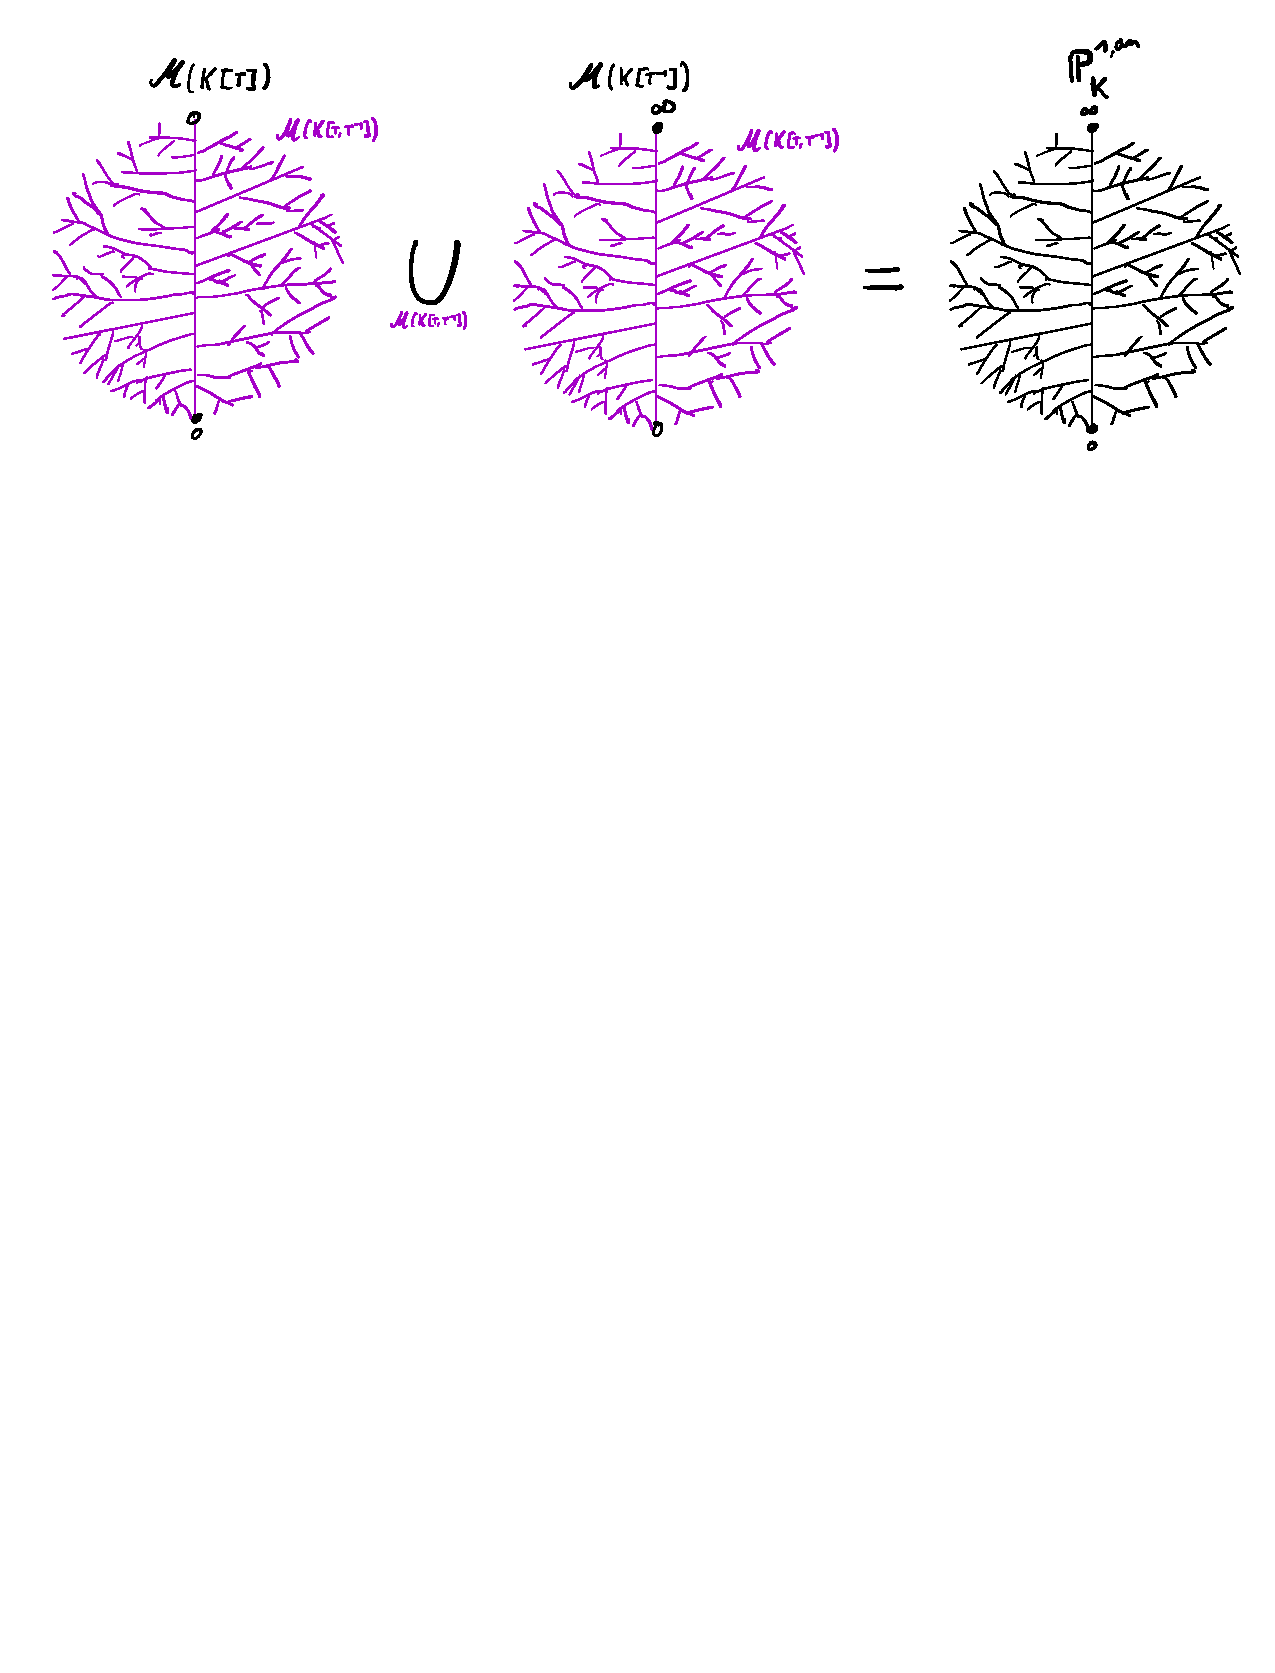
\includegraphics[width=\textwidth]{figures/projective_line}
	\caption{The Berkovich projective line constructed by gluing two copies of $\aff^{1, \text{an}}_K$}
	\label{fig:berk_projective_line}
\end{figure}


Like the analytification of complex varieties there are certain GAGA results, which show that under specific conditions all information is preserved by passing to the Berkovich analytification. 
Once one has setup the right definitions of smooth, flat, unramified, étale and open immersion for $K$-analytic spaces (see \cite[][sec. 3.1]{berkovichSpectralTheoryAnalytic2012} for definitions) one can show the following:
\begin{theorem}
	Let $f: Y \to X$  be a morphism of $K$-varieties. Then $f\an: Y \an \to X\an$ has any of the following properties if and only $\phi$ has: flat, unramified, étale, smooth, separated, injective, surjective, open immersion, isomorphism and monomorphism. 

	If moreover $f$ is a morphism of finite type then the following may be added to the list: dominant, closed immersion, proper and finite. 
\end{theorem}
\begin{proof}
	See \cite[][prop.\ 3.4.6 and prop.\ 3.4.7]{berkovichSpectralTheoryAnalytic2012}
\end{proof}

\begin{theorem}
	The topology of $X\an$ reveals a lot of the ``topological'' properties of the scheme $X$. 
	\begin{itemize}
		\item $X$ is separated if and only if $X\an$ is Hausdorff. 
		\item $X$ is proper if and only if $X\an$ is Hausdorff and compact. 
		\item  $X$ is connected if and only if $X\an$ is path-connected. 
		\item The Krull dimension of  $X$ is equal to the topological dimension of $X\an$. 
	\end{itemize}
\end{theorem}
\begin{proof}
	See \cite[][thm.\ 3.4.8]{berkovichSpectralTheoryAnalytic2012}
\end{proof}

For more on the GAGA results see \cite[][sec.\ 3.4]{berkovichSpectralTheoryAnalytic2012}.

\subsection{Generic fiber of a formal scheme} \label{sec:generic_fiber_of_a_formal_scheme}

Recall that $R = \mathcal{O}_K = \{a \in K \mid |a| \le 1\} $, which is a topological ring with the metric induced by the norm. 
Let $\pi$ be a pseudo-uniformiser for $R$ and $I = (\pi)$. 
Then $\{I^{n}\}_n$ gives a system of neighborhoods around zero, and $R$ is complete with respect to this topology. 
This means that $R$ is an adic ring, which is useful if we want to use the language of formal schemes. 

We first need to restrict the class of rings and formal schemes we consider. 
\begin{definition}\label{def:topologically_finite_presentation_algebra}
	\begin{itemize}
		\item 
	A \emph{topologically finitely presented} $R$-algebra is a quotient \[
		R\left<x_1, \ldots, x_n \right> / \mathfrak{a} 
	,\] where $\mathfrak{a}  = (f_1, \ldots, f_m)$ is a finitely generated ideal. 
\item A formal scheme that is locally isomorphic to $\spf A$ for some topologically finite presented $R$-algebra is called a \emph{locally finite type} $R$ formal scheme. 
	\end{itemize}

\end{definition}

Given such a topologically finitely presented ring $A = \frac{R \left<x_1, \ldots, x_n \right>}{(f_1, \ldots, f_m)}$ we can tensor it with $K$ to get its ``generic fiber'' which is an affinoid algebra \[
A \otimes _R K = \frac{K \left<x_1, \ldots, x_n \right>}{(f_1, \ldots, f_m)}
.\]  
This suggest the following functor $\spf A \mapsto \mathcal{M} (A \otimes_R K)$. 
Indeed this functor glues to give a functor from the topologically finitely presented $R$ formal schemes to the category of $K$-analytic spaces. 

\begin{definition}\label{def:generic_fibre_of_formal_scheme}
Given a topologically finitely presented formal schemes $\mathfrak{X} $ we call the resulting $K$-analytic space the \emph{generic fibre of  $\mathfrak{X} $} and denote it by $\mathfrak{X} _\eta$. 
\end{definition}

\begin{definition}
	Let $X$ be a $K$-variety. 
	\begin{itemize}
		\item A formal model of $X$ is a locally finite type formal $R$-scheme together with an isomorphism $X\an \cong \mathfrak{X}_{\eta}$.
		\item A formal model $\mathfrak{X}  $ of $X$ is \emph{semistable} if its special fiber $\mathfrak{X} _s = \mathfrak{X} \times_R \spec k$ is a connected reduced curve whose singularities are ordinary double points. 
	\end{itemize}
\end{definition}

\begin{comment}
Later we will extend the construction of the generic fiber to the larger class of \emph{special formal schemes}.
These will be really useful for understanding the relation between formal models of curves and their Berkovich space. 
\begin{definition}\label{def:special_r_algebra}
	A \emph{special} $R$-algebra is a $R$-algebra of the form \[
		\frac{A\left<x_1, \ldots, x_n \right>[[y_1, \ldots, y_m]]}{(f_1, \ldots, f_\ell)}
	.\] 
\end{definition}
\end{comment}








\section{Analytification of Curves} \label{sec:analytification_of_curves}


\section{What comes next} \label{sec:what_comes_next}

Tate elliptic curves

\printbibliography
\end{document}
